\documentclass[a4paper,12pt, twoside, russian]{report}
\usepackage{cmap}
\usepackage[T2A]{fontenc}
\usepackage[utf8x]{inputenc}
%\usepackage{cyrnewcent}
%\usepackage{lmodern}
\usepackage[russian]{babel}
\usepackage[unicode, pdftex,bookmarks=true,breaklinks=true]{hyperref}
%\usepackaghe{lh}
%\usepackage{cyrillic}
\usepackage{indentfirst}
\usepackage{ucs} 
\usepackage{graphicx}
\usepackage{wrapfig}

\hypersetup{
    colorlinks,
    citecolor=black,
    filecolor=black,
    linkcolor=blue,
    urlcolor=blue,
    pdftitle={Курс молодого бойца Vyatta},
    pdfauthor={Даниил Батурин <daniil@baturin.org>},
    %linktocpage
}

 \textwidth=16cm
 \textheight=25cm
 \oddsidemargin=-0.1cm
 \evensidemargin=0.11cm
 \headheight=0cm
 \topmargin=-1cm

\parindent=1cm

\emergencystretch=5pt


 % Заголовок документа
 \title{Курс молодого бойца Vyatta}
 \date{10 апреля 2011, версия 1.2}
 \author{Даниил Батурин}

\begin{document}
 \maketitle

\newcommand{\command}[1]{\texttt{#1}}

\tableofcontents
\addcontentsline{toc}{chapter}{Оглавление}

\chapter{Общие слова}

\section{Вместо предисловия}
На написание этого руководства меня вдохновил <<Курс молодого бойца Cisco>> Сергея (Fedia) Федорова. 
Надеюсь, что оно окажется полезным для начинающих пользователей. 

Документации, особенно русскоязычной, по вьятте пока что катастрофически мало, и этот 
документ призван хоть немного это исправить. Во многом он основан на материале публикаций в блогах AntiCisco.

Этот документ актуален для версии 6.4 и выше. Иногда встречаются указания на то, в какой версии появилась
функция.

Документ распространяется по лицензии CC-BY-SA, то есть, разрешается его использование в любых целях,
распространение и создание производных работ  при условии указании авторства и распространения производных 
работ под той же лицензией.

Последняя версия этого документа доступна по адресу \url{http://baturin.org/files/vb/vyatta_bootcamp.pdf}.
Если кто-то предлагает вам этот же документ в электронном или печатном виде за деньги, то автор к этому
никакого отношения не имеет и никакой прибыли с этого не получает.

Исходный код последней версии можно получить по адресу: \url{http://baturin.org/files/vb/vyatta_bootcamp_src.zip}

Сценарии настройки и прочие утверждения по возможности проверены на тестовых стендах, но автор, по понятным
причинам, не может ничего гарантировать. А также не отвечает за последствия применения его советов.

Связаться с автором можно по почте \href{mailto:daniil@baturin.org}{daniil@baturin.org}, желательно, указав в теме
<<КМБ Vyatta>>.

\subsubsection{Типографские соглашения}
\command{Моноширинным шрифтом} обозначены команды и их вывод. \\
В \textless угловых скобках\textgreater\ указаны обязательные аргументы команд. \\
В [квадратных скобках] указаны необязательные аргументы команд.

\section{Где взять?}
Последняя версия Vyatta доступна для скачивания на официальном сайте: 
\url{http://vyatta.org/downloads}.

Существуют три версии: Core, Subscription и Plus. Последние две можно получить только по платной подписке,
они отличаются наличием дополнительных компонентов (например, TACACS+, коммерческие наборы правил фильтрации URL и т.д.).

У всех версий есть разные варианты сборки. Выбор сборки зависит от того, куда вы собираетесь устанавливать 
систему. Есть следующие варианты:
\begin{itemize}
 \item[---] Live CD ISO --- предназначен для физических систем, может быть также установлен в любой
            гипервизор, кроме Xen в паравиртуальном режиме.
 \item[---] Virtialization ISO --- содержит паравиртуальное ядро для Xen и дополнения для VMWare.
\end{itemize}

Официально поддерживаются VMWare, Xen, XenServer и KVM. Драйверы virtio для KVM присутствуют в обоих вариантах образа,
поскольку являются частью ядра. Кроме упомянутых гипервизоров проверена также работа в VirtualBox и Parallels Desktop, проблем не замечено.

По адресу \url{ftp://ftp.het.net/iso/vyatta/} располагается собранная пользователями почти полная коллекция предыдущих версий и
документации к ним. Там же, в каталогах с именами веток, а не названиями версий (oxnard, pacifica и т.д.) находятся неофициальные
сборки находящихся в разработке версий. Так что если вы хотите заглянуть в прошлое или в будущее, то вам туда. Связаться с
держателями коллекции можно по адресу \href{mailto:unofficial@vyattawiki.net}{unofficial@vyattawiki.net}. Если у вас есть старые версии или документы, которых там нет,
они будут рады их включить.

\section{Где получить помощь?}
На форуме (\url{http://vyatta.org/forum}), на канале \command{$\sharp\sharp$vyatta} сети Freenode. Оба на 
английском языке, про IRC еще нужно учитывать, что большинство участников из США, 
а когда у них день --- у нас ночь.

\par\noindent Официальную документацию можно скачать на \url{http://vyatta.org/documentation}

\par\noindent На русском можно спрашивать на \url{http://anticisco.ru}.

Дополнительную информацию можно найти в неофициальной вики: \url{http://vyattawiki.net}.

\chapter{Искусство владения консолью}
\section{Основы}
Основным средством настройки Vyatta является консоль.Больше всего она похожа на консоль устройств Juniper Networks, и совсем не похожа на Cisco.
В Subscription Edition есть и графический веб-интерфейс, но консоль все равно удобнее и эффективнее.

Настройки имеют иерархическую структуру и представляют собой дерево с узлами и листями. Каждая команда
содержит модификатор операции, путь к нужному узлу и значение. Например:
\begin{verbatim}
set system name-server 192.0.2.1
\end{verbatim}
Здесь \command{set} --- модификатор, \command{system name-server} --- путь, \command{192.0.2.1} --- значение.

Основные модификаторы операций:
\begin{itemize}
 \item[---] \command{set} --- создать или изменить узел;
 \item[---] \command{delete} --- удалить узел.
\end{itemize}

Другие модификаторы будут рассмотрены позже. Они позволяют добавлять комментарии, а также копировать и
переименовывать узлы.

Интерфейс имеет два режима: режим операций и режим настройки. Сразу после входа вы попадаете в режим операций,
перейти в режим настройки можно командой \command{configure}. Выйти обратно можно командой \command{exit}.
Режимы легко отличить по приглашению командной строки: в операционном оно заканчивается <<\verb $ >>, в
настроечном --- <<\verb # >>.

Важно помнить, что команды не применяются сразу после их ввода. Чтобы их применить, нужно ввести команду
\command{commit}. Или отменить изменения командой \command{discard}.

Оцпиально можно указать краткое описание своих изменений командой
\begin{verbatim}
commit comment "<COMMENT TEXT>"
\end{verbatim}

Также можно обезопасить себя, если изменения потенциально могут заблокировать доступ к системе в случае
ошибки. Нужно ввести команду 
\begin{verbatim}commit-confirm [MINUTES]\end{verbatim}, и если в течении указанного времени 
(по умолчанию --- десять минут) не будет введена команда \command{confirm}, система автоматически вернется
к последней сохраненной конфигурации.
\par\noindent После завершения сеанса настроек нужно сохранить конфиг командой \command{save}. \\
\par\noindent Приведем несколько полезных приемов. \\

\par\noindent \textbf{Хитрость 1:} Используйте сочетания клавиш.
\begin{itemize}
 \item[---] Ctrl-A --- переход к началу строки;
 \item[---] Ctrl-E --- переход к концу строки;
 \item[---] Ctrl-W --- удалить слово назад;
 \item[---] Ctrl-U --- удалить всю строку;
 \item[---] Ctrl-K --- удалить все после курсора;
 \item[---] Alt-B --- переместить курсор на слово влево;
 \item[---] Alt-F --- переместить курсор на слово вправо;
 \item[---] Ctrl-C --- прервать текущий процесс (например, вывод логов);
 \item[---] Q --- выйти из просмотрщика (при просмотре текста, разделенного на экраны);
 \item[---] Ctrl-L --- очистить экран.
\end{itemize}
По истории команд можно перемещаться стрелками вверх и вниз.


\par\noindent \textbf{Хитрость 2:} Используйте автодополнение команд. По нажатию Tab команда либо дополняется 
(если введенная часть ее однозначно определяет), либо выводится список вариантов.


\par\noindent \textbf{Хитрость 3:} Выполнить команду операционного режима (вроде \command{show ip route}) 
из настроечного можно указав перед командой слово \command{run}. Например, 
\begin{verbatim}run show ip route\end{verbatim}


\par\noindent \textbf{Хитрость 4:} Можно просматривать не весь конфиг, а только интересующую часть.
Например, \begin{verbatim}show service dhcp-server\end{verbatim}

\par\noindent \textbf{Хитрость 5:} Чтобы не писать длинные команды, можно перейти на нужный уровень вложенности и
писать команды с относительным путем. Сравните:
\begin{verbatim}
set nat destination rule 10 protocol tcp
set service nat rule 10 source address 192.168.0.0/24
\end{verbatim}
и
\begin{verbatim}
edit nat destination rule 10
set protocol tcp
set source address 192.168.0.0/24
\end{verbatim}

\par\noindent \textbf{Хитрость 6:} По дереву настроек можно перемещаться командами \command{top} --- перейти
на верхний уровень и \command{up} --- перейти на один уровень выше. 

\par\noindent \textbf{Хитрость 7:} Используйте фильтры для получения нужной информации.
Доступны следующие фильтры:
\begin{itemize}
 \item[---] \command{|more} --- принудительно разделять вывод на экраны;
 \item[---] \command{|no-more} --- не разделять вывод на экраны;
 \item[---] \command{|match <KEYWORD>} --- вывести строки, содержащие слово \command{KEYWORD}. Можно писать
выражение из нескольких слов, если заключить его в кавычки. Также можно писать регулярные выражения;
 \item[---] \command{|no-match <KEYWORD>} --- вывести строки, не содержащие \command{KEYWORD};
 \item[---] \command{|count} --- напечатать число строк в выводе команды.
\end{itemize}

Фильтры можно комбинировать между собой, например узнать число правил destination NAT:
\begin{verbatim}
show nat destination|match rule|count
\end{verbatim}

Нужно заметить, что пробелы вокруг <<|>> допустимы, но не обязательны, в отличие от IOS.

\par\noindent \textbf{Хитрость 8:} По умолчанию нажатие <<?>> вызывает встроенную справку. Если нужно набрать
символ вопросительного знака, нужно сначала нажать Ctrl-V, а потом <<?>>.

\par\noindent \textbf{Хитрость 9:} Чтобы ввести строку с пробелами, заключите ее в двойные кавычки. Вроде
\begin{verbatim}
set nat destination rule 10 description "This is a NAT rule"
\end{verbatim}

Включать кавычки внутрь текстовых строк нельзя.

\section{Общие рекомендации}

\subsubsection{Имена}
Используйте осмысленные и единообразные имена конструкций (наборов правил МСЭ, route-map'ов и так далее). В этом
случае гораздо проще разобраться в том, что для чего нужно. Особенно это актуально для конфигов, написанных 
кем-то другим или просто долгое время назад.

Для повышения читаемости стоит писать все имена с заглавной буквы или целиком заглавными буквами --- в этом
случае их проще отличить от служебных слов.

\subsubsection{Комментарии}
Оставляйте комментарии к конструкциям. У большинства конструкций конфига есть параметр \command{description},
в котором можно оставить произвольный текст.

Добавить комментарий к произвольному месту конфига можно с помощью команды \command{comment}. Например,
\begin{verbatim}
comment protocols static route 192.168.42.0/24 "Route to remote office"
commit
\end{verbatim}
даст
\begin{verbatim}
 static {
     /* Route to remote office */
     route 192.168.42.0/24 {
         next-hop 192.168.42.1 {
         }
     }
\end{verbatim}
Удалить комментарий можно такой же командой, но с \verb ""  в качестве аргумента.

\subsubsection{Операции над конструкциями конфига}
Для экономии времени можно копировать и переименовывать конструкции. Делается это командами \command{copy} и
\command{rename}. Помните, что переименовать конструкцию, которая куда-то применена, не получится.

Для применения этих операций нужно перейти на уровень выше, чем находятся наши конструкции. Например, нам лень
писать два почти одинаковых правила NAT, отличающихся только портом назначения. Вот что можно сделать:
\begin{verbatim}
vyatta@vyatta# show nat destination
 rule 10 {
     destination {
         port http
     }
     inbound-interface eth0
     translation {
         address 10.91.17.100
         port http
     }
     protocol tcp
 }
[edit]
vyatta@vyatta# edit nat destination
[edit nat destination]
vyatta@vyatta# copy rule 10 to rule 20
[edit nat destination]
vyatta@vyatta# commit
[edit nat destination]
vyatta@vyatta# set rule 20 destination port https
vyatta@vyatta# set rule 20 inside-address port https
\end{verbatim}

\subsubsection{И еще}
Vyatta это надстройка над Debian GNU/Linux, и этого никто не скрывает. Но настраивать ее нужно через родной
интерфейс. Изменения, сделанные в конфигах из \command{/etc} вручную будут утеряны при следующем commit'е или перезагрузке.

Не стоит вносить изменения в настройки бэкендов, если только вы не знакомы с исходным кодом и внутренним устройством системы.
Если вы точно уверены в том, что делаете, можно осторожно добавить их в \command{/config/scripts/vyatta-postconfig-bootup.script}
Этот скрипт выполняется после загрузки настроек. Писать в /etc/rc.local не стоит, в отличие от содержимого /config он не будет
перенесен в новую систему при обновлении образа.

Впрочем, знание UNIX поможет в отладке и понимании происходящего.

\chapter{Начальные настройки}
Перед началом активного использования маршрутизатора стоит настроить удаленное управление и прочие служебные
вещи.

Прежде всего стоит указать имя хоста, чтобы потом не сомневаться что именно за маршрутизатор мы настраиваем.
Оно отображается в приглашении командной строки и в логах. Указывается командой 
\begin{verbatim}set system host-name <NAME>\end{verbatim}

Нужно отметить, что в приглашении командной строки его станет видно только при следующем входе в систему.

\section{Дата и время}
Для удобства чтения логов можно настроить часовой пояс. По умолчанию используется UTC. В географически
распределенных системах советуют ставить для всего оборудования именно его. Поменять можно командой
\begin{verbatim}set system time-zone <REGION/CITY>\end{verbatim}
Например, Europe/Moscow. Нужный проще всего найти автодополнением.

Настраивать переход на летнее время не нужно, для часовых поясов, где он присутствует, перевод происходит
автоматически.

Также можно указать свои NTP-сервера командой \begin{verbatim}set system ntp server <HOSTNAME>\end{verbatim}
По умолчанию там уже присутствуют сервера [012].vyatta.pool.ntp.org.\footnote{Которые, вероятно, еще и собирают
анонимную статистику по географии установок. По крайней мере откуда-то она берется, а это самое логичное
предположение. Посмотреть можно тут: \href{http://kellyherrell.wordpress.com/2010/09/29/vyatta-network-os-officially-everywhere/}
{http://kellyherrell.wordpress.com/2010/09/29/vyatta-network-os-officially-everywhere/}}

\section{DNS}

Для удобства отладки можно настроить DNS-серверы командой \begin{verbatim}set system name-server <IPADDRESS>
\end{verbatim}

Также можно указать домен по умолчанию. Тогда если указан домен\\ \command{example.com}, 
при разрешении хоста вида
\command{host} будет предполагаться \\ \command{host.example.com}. Делается это командой:
\begin{verbatim}set system domain-name example.com\end{verbatim}

\section{Включаем удаленное управление}
К сетевому устройству логично иметь удаленный доступ по сети. Нам доступно три варианта:
\begin{itemize}
 \item[---] Telnet;
 \item[---] SSH;
\end{itemize}

Включить Telnet можно командой: \begin{verbatim}set service telnet\end{verbatim} Опциально можно изменить порт,
на котором он слушает: \begin{verbatim}set service telnet port <NUMBER>\end{verbatim}

SSH включается командой: \begin{verbatim}set service ssh\end{verbatim} Опциально также можно указать порт,
той же опцией, что у Telnet. Для генерации ключей ничего предпринимать не надо --- они сгенерируются автоматически.

\section{Заводим пользователей}
По умолчанию в системе есть только один пользователь --- vyatta, которого еще и нельзя удалить. Зато можно
завести новых. В этом случае можно будет:
\begin{itemize}
 \item[---] Видеть, кто именно сейчас подключен к системе;
 \item[---] Ограничить пользователю полномочия;
 \item[---] Найти ответственного за те или иные изменения настроек.
\end{itemize}

Добавление пользователя выглядит так:
\begin{verbatim}
edit system login user <NAME>
set authentication plaintext-password <PASSWORD>
set full-name "<FULL NAME>"
\end{verbatim}

Слова \command{plaintext-password} не надо бояться, оно значит лишь то, что пароль вводится в открытом виде.
При применении настроек он будет зашифрован. Если у вас уже есть хэш пароля (например, при переносе
пользователей с другой системы), можно вместо нее использовать \command{encrypted-password <HASH>}.

С помощью опции \command{set level operator} можно запретить пользователю вносить изменения в настройки.
<<Повысить>> пользователя потом будет можно сменой \command{operator} на \command{admin}.

\chapter{Пример настройки сети}
Теперь решим приближенную к реальной задачу. Предположим, что у нас есть сеть небольшой компании, в которой надо:
\begin{itemize}
 \item[---] Раздать рабочим станциям адреса по DHCP;
 \item[---] Обеспечить раздачу им Интернета;
 \item[---] Защитить сеть межсетевым экраном;
 \item[---] Прокинуть несколько портов на корпоративный сервер;
 \item[---] Обеспечить сотрудникам удаленный доступ к сети.
\end{itemize}

\begin{figure}[hc]
 \begin{center}
   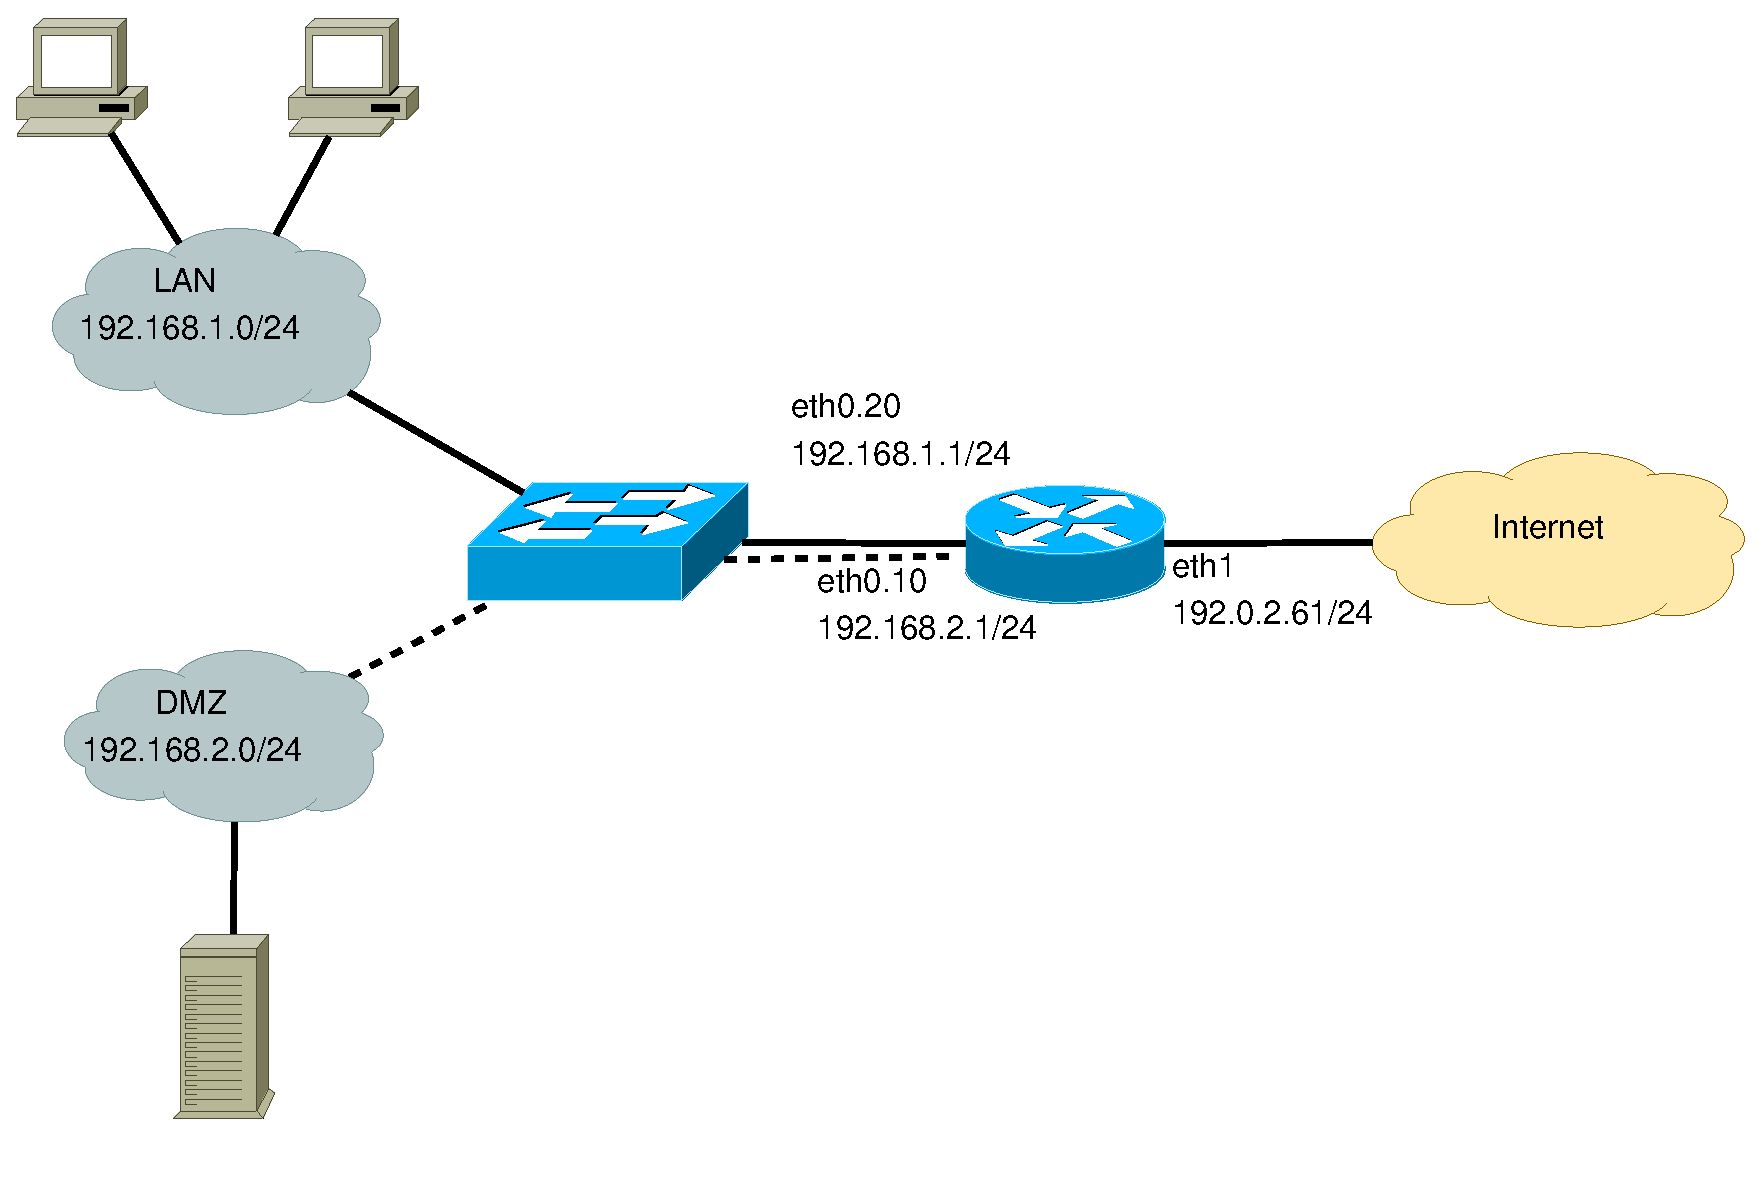
\includegraphics[width=0.7\textwidth]{images/topology}
   \caption{Топология сети}
  \end{center}
\end{figure}

Предположим также, что шлюз провайдера --- 192.0.2.1. Сеть поделена на два VLAN:
для рабочих станций (тег 20, с адресами 192.168.1.0/24) и для серверов (тег 10, 192.168.2.0/24).

\section{Настраиваем интерфейсы}
Пусть eth0 будет внутренним интерфейсом, а eth1 --- внешним. Начнем с внешнего и присвоим ему адрес:
\begin{verbatim}
configure
set interfaces ethernet eth1 address 192.0.2.61/24
commit
\end{verbatim}
Если провайдер использует DHCP, то вместо адреса нужно использовать опцию \command{dhcp}:
\begin{verbatim}
set interfaces ethernet eth1 address dhcp
\end{verbatim}

Теперь перейдем к внутреннему интерфейсу. На нем нужно создать два VLAN. Делается это следующим образом:
\begin{verbatim}
edit interfaces ethernet eth0
set vif 10 address 192.168.2.1/24
set vif 20 address 192.168.1.1/24
commit
\end{verbatim}

Посмотрим, что у нас получилось:
\begin{verbatim}
# show interfaces ethernet eth0
 duplex auto
 smp_affinity auto
 speed auto
 vif 10 {
     address 192.168.2.1/24
 }
 vif 20 {
     address 192.168.1.1/24
 }
\end{verbatim}

Также настроим маршрут по умолчанию:
\begin{verbatim}
set protocols static route 0.0.0.0/0 next-hop 192.0.2.1
\end{verbatim}


\section{Настраиваем DHCP}
Нам потребуются два пула адресов. Приступаем к настройке:
\begin{verbatim}
edit service dhcp-server shared-network-name LAN
set authoritative # Объявляем сервер ответственным за сеть
edit subnet 192.168.1.0/24
set start 192.168.1.100 stop 192.168.1.200 # Диапазон адресов
set default-router 192.168.1.1 # Шлюз по умолчанию
set dns-server 192.0.2.250 # DNS-сервер

top
edit service dhcp-server shared-network-name DMZ
set authoritative
edit subnet 192.168.2.0/24
set start 192.168.2.100 stop 192.168.2.200
set default-router 192.168.2.1
set dns-server 192.0.2.250
\end{verbatim}

Пусть нам нужно выдавать серверу фиксированный адрес 192.168.2.50. Пусть его сетевая карта имеет
MAC-адрес 00:aa:bb:cc:dd:ee. Создадим соответсвующее правило:
\begin{verbatim}
edit service dhcp-server shared-network-name DMZ
edit subnet 192.168.2.0/24
set static-mapping Server ip-address 192.168.2.50
set static-mapping Server mac-address 00:aa:bb:cc:dd:ee
\end{verbatim}

Посмотрим на получившуюся конфигурацию:
\begin{verbatim}
# show service dhcp-server 
 shared-network-name DMZ {
     subnet 192.168.2.0/24 {
         default-router 192.168.2.1
         dns-server 192.0.2.250
         start 192.168.2.100 {
             stop 192.168.2.200
         }
         static-mapping Server {
             ip-address 192.168.2.50
             mac-address 00:aa:bb:cc:dd:ee
         }
     }
 }
 shared-network-name LAN {
     subnet 192.168.1.0/24 {
         default-router 192.168.1.1
         dns-server 192.0.2.250
         start 192.168.1.100 {
             stop 192.168.1.200
         }
     }
 }
\end{verbatim}


\section{Настраиваем NAT}
Нам нужны два вида правил: одни будут транслировать внутренние адреса во внешние чтобы обеспечить внутренней
сети доступ в Интернет, вторые будут транслировать внешний адрес во внутренний чтобы обеспечить доступ снаружи
к серверу внутри.

Начнем с правил для раздачи Интернета:
\begin{verbatim}
edit nat source rule 10
set source address 192.168.1.0/24
set outbound-interface eth1
set translation address  masquerade
set description "LAN to the Internet"
top
\end{verbatim}
По аналогии создадим правило для второй сети:
\begin{verbatim}
edit nat source rule 20
set source address 192.168.2.0/24
set outbound-interface eth1
set translation address masquerade
set description "DMZ to the Internet"
top
\end{verbatim}

Теперь займемся пробросом портов внутрь. Пусть нам нужно пробросить порты  80 и 25.
\begin{verbatim}
edit nat destination rule 10
set destination port http
set protocol tcp
set inbound-interface eth1
set translation address 192.168.2.50
set translation port http
top
\end{verbatim}
Правило про порт 25 отличается только опцией \command{port}.

Смотрим результат:
\begin{verbatim}
#show nat 
destination {
    rule 10 {
        destination {
            port http
        }
        inbound-interface eth1
        protocol tcp
        translation {
            address 192.168.2.50
            port http
        }
    }
    rule 20 {
        destination {
            port smtp
        }
        inbound-interface eth1
        protocol tcp
        translation {
            address 192.168.2.50
            port smtp
        }
    }
}
source {
    rule 10 {
        description "LAN to the Internet"
        outbound-interface eth1
        source {
            address 192.168.1.0/24
        }
        translation {
            address masquerade
        }
    }
    rule 20 {
        description "DMZ to the Internet"
        outbound-interface eth1
        source {
            address 192.168.2.0/24
        }
        translation {
            address masquerade
        }
    }
}
\end{verbatim}

Обратите внимание, что вместо номеров портов можно указывать их названия, как в нашем примере указан 
\command{http} вместо 80. Полный список можно получить командой 
\begin{verbatim}
cat /etc/services
\end{verbatim}

\section{Настраиваем удаленный доступ по PPTP}
Чтобы обеспечить нашим пользователям возможность удаленного подключения к корпоративной сети, мы настроим
доступ по PPTP. Протокол далеко не самый удачный и безопасный, но зато прост в настройке как на маршрутизаторе,
так и на клиентах.
\begin{verbatim}
edit vpn pptp remote-access
set client-ip-pool start 192.168.3.1
set client-ip-pool stop 192.168.3.50
set dns-servers server-1 192.168.2.50
set authentication mode local
set authentication local-users username User password 2WsX3EdC
\end{verbatim}
Для минимальной работы этого достаточно. 

\section{Настраиваем МСЭ}
В современном Интернете так много угроз безопасности, что оставлять сеть незащищенной --- преступная халатность.
Поэтому мы настроим фильтрацию трафика с помощью МСЭ. В первую очередь сформулируем задачу. Нам нужно:
\begin{itemize}
 \item[---] Разрешить установку соединений изнутри сети куда угодно;
 \item[---] Разрешить подключения к корпоративному серверу по HTTP (порт TCP/80) и SMTP (TCP/25);
 \item[---] Разрешить подключения к маршрутизатору по протоколу PPTP (порт TCP/1723 и протокол GRE);
 \item[---] Разрешить исходящие соединения из сети рабочих станций в сеть серверов, но не наоборот;
 \item[---] Разрешить исходящие соединения по протоколу SMTP (TCP/25) в Интернет только корпоративному серверу;
 \item[---] Запретить все остальное.
\end{itemize}

Приступаем. Идеология настройки такова: мы создаем наборы правил фильтрации, а потом применяем их к
сетевым интерфейсам. У каждого интерфейса могут быть наборы правил для трех направлений:
\begin{itemize}
 \item[---] \command{in} --- соединения снаружи внутрь сети;
 \item[---] \command{out} --- соединения изнутри сети наружу;
 \item[---] \command{local} --- соединения к самому маршрутизатору.
\end{itemize}

Нам потребуются четыре набора правил: из Интернета во внутреннюю сеть, из Интернета к маршрутизатору, из
сети серверов (192.168.2.0/24) в сеть рабочих станций (192.168.1.0/24) и из локальной сети в Интернет.
Назовем их, соответственно,
\command{Inet-Local}, \command{Inet-Router}, \command{DMZ-LAN} и \command{Local-Inet}.

\subsubsection{Создаем Inet-Local}

В нем нам нужно разрешить входящие соединения на TCP/80 и TCP/25, а также те соединения, которые
уже были установлены изнутри сети.

\begin{verbatim}
edit firewall name Inet-Local

set rule 10 action accept
set rule 10 state established enable
set rule 10 state related enable

set rule 20 action accept
set rule 20 destination port http
set rule 20 protocol tcp

set rule 30 action accept
set rule 30 destination port smtp
set rule 30 protocol tcp
\end{verbatim}

Первое правило требует некоторых пояснений. Vyatta умеет отслеживать состояния соединений и запоминать их.
Состояний бывает четыре: \command{new} --- устанавливаемые соединения, \command{established} --- уже установленные,
\command{related} --- соединения, являющиеся вспомогательными для уже установленных (такие возникают, например,
в протоколе FTP, который использует разные соединения для управления и для передачи данных) и \command{invalid}
--- не попадающие ни под один из указанных критериев.

Таким образом, этим правилом мы разрешили прохождение во внутреннюю сеть трафика, который соответствует соединениям,
которые уже были установлены изнутри и вспомогательных к ним.

\subsubsection{Создаем Inet-Router}
\begin{verbatim}
edit firewall name Inet-Router

set rule 10 action accept
set rule 10 state established enable
set rule 10 state related enable

set rule 20 action accept
set rule 20 destination port 1723
set rule 20 protocol tcp

\end{verbatim}
Вопрос, который он может вызвать: почему мы разрешили порт управляющего соединения PPTP, но не разрешили GRE,
который он использует для передачи данных? Все потому, что это соединение будет в состоянии \command{related} 
по отношению к управляющему, а первое правило его разрешает.

\subsubsection{Создаем DMZ-LAN}
\begin{verbatim}
edit firewall name DMZ-LAN

set default-action accept

set rule 10 action drop
set rule 10 destination address 192.168.1.0/24
set rule 10 state new enable
\end{verbatim}

Этим набором правил мы разрешили все, кроме установки соединений в сеть рабочих станций. Обратите внимание на
опцию \command{default-action}. Ей можно поменять действие, которое применяется к трафику, который не соответствует ни
одному из правил. По умолчанию оно установлено в \command{drop}.

\subsubsection{Создаем Local-Inet}
Если рабочие станции наловят рассылающих спам червей, нам грозит попадание внешнего адреса в черные списки,
выбираться из которых довольно утомительно. Поэтому мы запретим SMTP-соединения для всех машин, кроме
корпоративного сервера.

\begin{verbatim}
edit firewall name Local-Inet

set default-action accept

set rule 10 action drop
set rule 10 destination port smtp
set rule 10 source address !192.168.2.50
set rule 10 protocol tcp
\end{verbatim}

Обратите внимание на опцию \command{source address}. Символ \command{!} означает <<все, кроме указанного>>,
таким образом, правило запрещает SMTP для всех, кроме 192.168.2.50.

\subsubsection{Применяем наборы правил к интерфейсам}
Набор правил Inet-Local должен быть применен в направлении \command{in} внешнего интерфейса.
\begin{verbatim}
set interfaces ethernet eth1 firewall in name Inet-Local
\end{verbatim}

Набор правил Inet-Router нужно применить в направлении \command{local} внешнего интерфейса.
\begin{verbatim}
set interfaces ethernet eth1 firewall local name Inet-Router
\end{verbatim}

Набор DMZ-LAN нужно применить в направлении \command{in} того интерфейса, который смотрит в сеть с серверами.
\begin{verbatim}
set interfaces ethernet eth0 vif 10 firewall in name DMZ-LAN
\end{verbatim}

Набор Local-Inet нужно применить в направлении \command{out} внешнего интерфейса.
\begin{verbatim}
set interfaces ethernet eth1 firewall out name Local-Inet
\end{verbatim}

Теперь наша сеть относительно защищена.

\chapter{Работа с конфигурацией}
\section{Немного теории}
Для начала посмотрим, как именно вьятта работает со своими настройками. Каждый конфиг проходит
в своей жизни три стадии: 
\begin{itemize}
 \item[---] Рабочая копия (working);
 \item[---] Действующий конфиг (active);
 \item[---] Сохраненный конфиг.
\end{itemize}

Рабочая копия это то, что получается когда пользователь внес изменения, но еще не применил их.
На каждую сессию (на вход пользователя или работу скрипта) создается своя рабочая копия. 
У нее два варианта дальнейшей жизни: быть объединенной с действующей (командой \command{commit})
или быть отброшенной.

Действующий конфиг это, очевидно, тот, который система в настоящий момент использует.

Сохраненный конфиг это простой текстовый файл. По умолчанию они хранятся в каталоге 
\command{/config/}.

Для тех, кому интересно, как рабочая и действующая копии конфига устроены внутри. 
Это деревья каталогов в \command{/opt/vyatta/config/active} (для действующего) и 
\command{/opt/vyatta/config/tmp/*}
(для рабочих копий). Узлу, например, \command{service telnet port} там соответствует каталог
\command{service/telnet/port}. Значение для узла хранится в файле \command{node.val}.

Трогать это все руками не рекомендуется, если только не для изучения внутреннего устройства системы.

\section{Делаем копии конфига}

Получить копию действующего конфига на стандартный вывод можно командой \command{show|no-more}.
В этом случае он будет показан целиком, без разделения на экраны, как это происходит по умолчанию.

Сохраненные конфиги это простые текстовые файлы. Тот, который загружается по умолчанию, называется 
\command{/config/config.boot}. Командой \command{save} с аргументом, вроде 
\begin{verbatim}save config-2012.04.01\end{verbatim}
можно сохранить его под другим именем.

Загрузить ранее сохраненный конфиг можно командой \begin{verbatim}load <FILE NAME>\end{verbatim}
Также можно загружать его по сети, указав URL Например, 
\begin{verbatim}load ftp://example.com/config.txt\end{verbatim}

Так же можно и сохранять конфиг на удаленный сервер, указав целевой URL. Например, 
\begin{verbatim}save tftp://192.0.2.1/config.boot\end{verbatim}

Кроме этого, в системе есть файл, который хранит настройки по умолчанию (которые использует 
свежеустановленная система), называется он \\ \command{/opt/vyatta/etc/config.boot.default}.
Соответственно, загрузив его, можно вернуться к начальным настройкам.

\section{Копируем кусок конфига с другой системы}

Тут есть два варианта. Первый по идеологии напоминает Cisco и состоит в получении команд текущего
конфига и вставке их в консоль целевой системы. Просмотреть команды можно с помощью команды операционного
режима \begin{verbatim}show configuration commands|match <KEYWORD>\end{verbatim}, 
где \command{KEYWORD} --- слово для выборки, например, \command{service ssh}.
\begin{verbatim}
# run show configuration commands |match "service ssh"
set service ssh port '22'
set service ssh protocol-version 'v2'
\end{verbatim}

Второй состоит в слиянии двух файлов конфигурации командой \command{merge}. Для этого нужно подготовить файл с нужным
куском настроек, перенести его на целевую систему (или положить в доступное по сети место) и ввести команду
\begin{verbatim}merge /path/to/file\end{verbatim} Вам выдадут предупреждение об отсутствиии строки версии
(если вы не скопировали ее из оригинального конфига, это самая последняя строка), но его можно игнорировать.

\section{Автоматизируем резервное копирование}

Начиная с версии 6.2 появилась возможность автоматически делать резервную копию конфига после каждого commit’а.
Делается это следующим образом: 
\begin{verbatim}set system config-management commit-archive location <URL>\end{verbatim} Например:
\begin{verbatim}
# show system config-management
 commit-archive {
     location ftp://10.91.17.5/pub/configs
 }
\end{verbatim}
Все, теперь каждый раз, когда вы применяете свои изменения, ваш конфиг будет копироваться в указанное
место под именем вида \\ \command{config.boot-yourhostname.yyyymmdd\_hhmmss}.

Поддерживается сохранение по TFTP, FTP и SCP.

\section{Ищем виноватых}

Начиная опять же с 6.2 каждый commit оставляет свой след в истории, и даже сохраняются тексты разных ревизий 
конфига. Настроить количество ревизий для хранения можно командой:
\begin{verbatim}set system config-management commit-revisions <NUMBER>\end{verbatim}

Командой операционного режима \begin{verbatim}show system commit\end{verbatim}
можно увидеть имеющиеся ревизии. Примерно так:
\begin{verbatim}
# run show system commit
0   2011-04-01 00:20:36 by vyatta via cli
1   2011-04-01 00:08:30 by user1 via cli
2   2011-04-01 00:03:16 by user2 via cli
3   2011-04-01 00:01:52 by user3 via cli
\end{verbatim}

Можно посмотреть либо конфигурацию целиком, как она выглядела на момент ревизии с некоторым номером по
команде \begin{verbatim}show system commit file <NUMBER>\end{verbatim} либо ее отличия от текущей командой 
\begin{verbatim}show system commit diff <NUMBER>\end{verbatim} Например:
\begin{verbatim}
# run show system commit diff 0
@@ -110,7 +110,7 @@
     console {
     }
     domain-name example.com
-    host-name dut1
+    host-name r1
     login {
         user vyatta {
             authentication {
@@ -121,8 +121,6 @@
     }
     name-server 10.91.17.10
     ntp {
-        server 0.vyatta.pool.ntp.org {
-        }
         server 1.vyatta.pool.ntp.org {
         }
         server 2.vyatta.pool.ntp.org {
\end{verbatim}
Появившиеся в ревизии строки отмечены символом «+», убранные в ней, соответственно, символом «-». 

\chapter{Отладка и поиск неисправностей}

Vyatta располагает достаточно большим набором средств отладки и диагностики, которые помогают понять, 
что именно идет не так. Здесь я описываю, по возможности, только штатные (присутствующие в родном CLI) 
средства, хотя ничто не мешает использовать произвольные инструменты Linux. 

\section{Системные сообщения}

Первое, с чего стоит начинать поиск. Сообщения (логи) вполне информативны, и часто одних их вполне достаточно.
Смотреть их можно командой операционного режима \command{show log}, имеющей ряд аргументов. 
\command{show log tail} покажет только последние десять строк. А если применить ее
с целым числом в качестве аргумента, вроде \command{show log tail 20}, то покажет указанное число строк.
\begin{verbatim}show log all\end{verbatim} покажет все накопившиеся сообщения.

Зачастую бывает полезно смотреть логи по мере их поступления. Это можно сделать командой \command{monitor log}.

Типичный формат сообщения таков: \begin{verbatim}[дата и время] [компонент]: [сообщение]\end{verbatim}
Например,
\begin{verbatim}Apr 1 06:39:30 vyatta vyatta-zebra[1923]: interface vtun6 index 602
deleted
\end{verbatim}

Кроме того, для некоторых типов интерфейсов можно посмотреть сообщения, касающиеся исключительно их 
(например, для PPPoE).
\begin{verbatim}
$show interfaces pppoe pppoe0 log
Wed Mar 24 14:43:46 NOVT 2011: PPP interface pppoe0 created
Wed Mar 24 14:44:01 NOVT 2011: Stopping PPP daemon for pppoe0
Wed Mar 24 14:44:02 NOVT 2011: Starting PPP daemon for pppoe0
Serial connection established.
\end{verbatim}

Для выхода из просмотра сообщений используйте cочетание клавиш Ctrl-C.

\section{Соединения и проходящий трафик}

Просмотреть активные соединения можно командой \begin{verbatim}show system connections\end{verbatim}
Выглядеть будет примерно так:
\begin{verbatim}
Active Internet connections (servers and established)
Proto Recv-Q Send-Q Local Address         Foreign Address     State
tcp        0      0 0.0.0.0:179           0.0.0.0:*           LISTEN     
tcp        0      0 10.55.6.3:179         10.55.6.4:59153     SYN_RECV   
tcp        0      0 0.0.0.0:1723          0.0.0.0:*           LISTEN     
tcp        0      0 192.0.2.10:9755       0.0.0.0:*           LISTEN     
tcp        0      0 192.0.2.10:9756       0.0.0.0:*           LISTEN     
tcp        0      0 0.0.0.0:222           0.0.0.0:*           LISTEN     
tcp        0      0 192.0.2.10:1723   198.51.100.3:30279  ESTABLISHED
tcp        0      0 192.0.2.10:1723   198.51.100.4:50556 ESTABLISHED
tcp        0      0 192.0.2.10:1723   198.51.100.5:32393  ESTABLISHED
tcp        0      0 192.0.2.10:1723   198.51.100.6:32023  ESTABLISHED
\end{verbatim}

Используя аргумент этой команды \command{tcp} или \command{udp} можно получить, соответственно, 
только TCP или только UDP соединения.

Кроме того, можно в реальном времени просматривать проходящий через интерфейс трафик командой 
\begin{verbatim}monitor interfaces <type> <name> traffic\end{verbatim} 
Там показывают весьма детальную статистику проходящих пакетов со сведениями о типе их содержимого
(а также адресами отправителя и получателя, флагами TCP и прочими полезными сведениями).
\begin{verbatim}
# run monitor interfaces ethernet eth1 traffic 
Capturing traffic on eth1 ...
  0.000000 192.0.2.10 -> 198.51.100.3 TCP 53456 > 32033 [SYN] Seq=0 Win=8192 Len=0 MSS=1460
  0.000377 72:1c:58:5e:94:7b -> ff:ff:ff:ff:ff:ff ARP Who has 198.51.100.210?  Tell 198.51.100.1
  0.019348 72:1c:58:5e:94:7b -> ff:ff:ff:ff:ff:ff ARP Who has 198.51.100.244?  Tell 198.51.100.1
  0.022846 72:1c:58:5e:94:7b -> ff:ff:ff:ff:ff:ff ARP Who has 198.51.100.98?  Tell 198.51.100.1
\end{verbatim}

Еще можно использовать аргументы \command{port PORTNUMBER} и \command{not port PORTNUMBER}
чтобы просмотреть пакеты только 
на определенный порт, или наоборот, на все кроме заданного (например, исключить порт 22 чтобы не видеть
соединение по SSH между собой и маршрутизатором).
К сожалению, для интерфейсов VPN-сессий так просмотреть трафик не получится: их просто нет в CLI. 
Но можно сказать \begin{verbatim}sudo tshark -i pppX\end{verbatim} и получить в точности то же самое.
У Wireshark (бывший Ethereal), который служит бэкендом захвата пакетов, есть еще графическая оболочка,
которой теоретически можно этот вывод скормить для более визуального просмотра и анализа. Я не пробовал, 
но если у кого будет желание, расскажите верно мое предположение или нет.

\section{Межсетевой экран}

Для проверки работы правил МСЭ можно посмотреть статистику командой 
\begin{verbatim}show firewall statistics\end{verbatim} или, для получения более подробных сведений, 
\begin{verbatim}show firewall detail\end{verbatim}
\begin{verbatim}
$show firewall statistics
IPv4 Firewall "InternetToLocal":
 Active on (eth1,IN)
rule  packets   bytes     action  source         destination
----  -------   -----    ------   ------         -----------
1     172.75M   78.48G    ACCEPT  0.0.0.0/0      0.0.0.0/0
10    0         0         ACCEPT  0.0.0.0/0      0.0.0.0/0
20    548.49K   30.16M    ACCEPT  0.0.0.0/0      0.0.0.0/0
25    222       11.37K    ACCEPT  0.0.0.0/0      0.0.0.0/0
-------------------------------------------------------------
\end{verbatim}

Как видно, вывод показывают отдельно по каждому набору правил МСЭ и правилу в нем. Для большей 
наглядности изменения счетчиков в процессе работы их можно предварительно сбросить командой 
\begin{verbatim}clear firewall <RULESET_NAME>\end{verbatim}

Если какие-то правила вызывают сомнения или просто мешают, можно отключить их с помощью опции
\command{disable (set firewall <RULESET\_NAME> rule <NUMBER> disable)}.

\section{NAT}

Процесс отладки трансляции сетевых адресов в целом напоминает то же с МСЭ. Можно просмотреть активные 
трансляции с помощью \begin{verbatim}show nat <source|destination> translations\end{verbatim}, статистику работы правил через 
\begin{verbatim}show nat <source|destination> statistics\end{verbatim} и сбросить счетчики командой 
\begin{verbatim}clear nat <source|destination> counters rule <NUMBER>\end{verbatim}
\begin{verbatim}
# run show nat source statistics 
rule   pkts    bytes   interface   
----   ----    -----   ---------   
10     545K    38M     eth1.115    
15     44470   3509K   pppoe0      
20     0       0       eth1.115    
30     37      2220    tun20       
\end{verbatim}

Неугодное правило трансляции можно отключить той же опцией \command{disable}: 
\begin{verbatim}set nat <source|destination> rule <NUMBER> disable\end{verbatim}

\section{Сетевые интерфейсы}

Для физических интерфейсов, например Ethernet, можно получить некоторые диагностические сведения.
Например, \begin{verbatim}show interfaces ethernet ethX statistics\end{verbatim}
покажет счетчики прошедших пакетов. Сбросить их можно путем 
\begin{verbatim}clear interfaces ethernet ethX counters\end{verbatim}
С помощью \begin{verbatim}show interfaces ethernet ethX physical\end{verbatim}
можно увидеть сведения о режиме работы интерфейса (поддерживаемые и текущая скорость передачи, дуплекс, 
наличие линка), используемый драйвер и прочее в этом духе. Параметр \command{bus-info} из вывод этой команды 
показывает номер слота шины, в котором он стоит, что может быть полезно для сопоставления имен интерфейсов
с сетевыми картами.

Для задачи поиска нужного интерфейса (а на произвольной машине это актуально, поскольку в отличие от
готовых решений подписей под ними нет) есть команда 
\begin{verbatim}show interfaces ethernet ethX identify\end{verbatim}, которая заставит выбранный интерфейс
моргать индикаторами. К сожалению, работает не для всех типов сетевых карт.

\section{Отладка протоколов маршрутизации}

Режим отладки можно включить командой \begin{verbatim}debug <PROTOCOL>\end{verbatim}, например, 
\begin{verbatim}debug ospf events\end{verbatim}, а просмотреть включена ли отладка с помощью 
\begin{verbatim}show debugging <PROTOCOL>\end{verbatim} Отладочные сообщения будут показаны в логах. 
Отключить обратно можно с помощью \begin{verbatim}no debug <PROTOCOL>\end{verbatim}

\section{Проблемы с самой системой}

Если с самим маршрутизатором произошло что-то страшное, либо просто хочется узнать подробности его жизни, 
можно использовать следующие команды:
\begin{itemize}
\item[---] Вполняющиеся процессы: \command{show system processes};
\item[---] Сообщения ядра в процеесе работы: \command{show system kernel-messages};
\item[---] Сообщения ядра во время загрузки: \command{show system boot-messages};
\item[---] Использование памяти: \command{show system memory}. С аргументом \command{quagga}
она выведет использования памяти стеком маршрутизации;
\item[---] Использование дискового пространства: \command{show system storage}
\item[---] Список устройств PCI: \command{show hardware pci}.
\end{itemize}

\end{document}
